\documentclass{../lab}

\labacronym{NLD}
\labtitle{Non-Linear Dynamics and Chaos}

%\newcommand{\ExperimentandProcedure}{http://experimentationlab.berkeley.edu/node/102}
%\newcommand{\Physics111LibrarySite}{http://physics111.lib.berkeley.edu/Physics111/Reprints/NLD/NLD_index.html}
%\newcommand{\(Ref.1,§11.5}{http://physics111.lib.berkeley.edu/Physics111/Reprints/NLD/Strogatz_Nonlinear_dynamics_chaos.pdf}

\begin{document}

\maketitle

\tableofcontents

\section{Non-Linear Dynamics and Chaos Description (NLD)}

\begin{enumerate}
    \item \textbf{Note that there is NO eating or drinking in the 111-Lab anywhere, except in rooms 282 \& 286 LeConte on the bench with the BLUE stripe around it.} Thank You, the Staff.
\end{enumerate}

\newpage

This experiment is an introduction to Non-Linear Dynamics, Data Acquisition, Chaos theory and Fractals. Limited as we are by our senses and relatively short powers of recall, much of the physical world seems aperiodic and defies quantitative description. While we have yet to discover closed form solutions to the simplest of systems (e.g. the one-dimensional gravitational three-body problem), the field of chaos reveals structure in their dynamics. The results of chaos theory have found practical applications in almost every branch of science.

In this experiment you will study the response of at least two different dynamical systems: A non-linear, damped harmonic oscillator and a system of op amps that reproduces the Lorentz attractor. You will measure their linear and non-linear behavior and write software to measure their information dimension.

You will learn the basics of digital sampling, Fourier transforms, geometric analysis of autonomous differential equations, information entropy, correlation dimension and the basics of programming in LabView (a data-acquisition and control language).

There are no pre-requisites. But a strong background in differential equations and classical mechanics, coupled with a willingness to do a lot of reading will serve you well in this lab.

\begin{enumerate}
    \item Pre-requisites: None

    \item Days Allotted for the Experiment: 7

\end{enumerate}

Pages of this lab.

\begin{enumerate}
    \item \textbf{Non-Linear Dynamics and Chaos} (here)

    \item \href{http://experimentationlab.berkeley.edu/node/102}{\textbf{Experiment and Procedure}}
    
    \item \href{http://experimentationlab.berkeley.edu/node/103}{\textbf{The custom VI's for this experiment \& Appendix}}
\end{enumerate}

This lab will be graded 40\% on theory, 20\% on technique, and 40\% on analysis. For more information, see the \href{\AdvancedLabSyllabus}{\textbf{Advanced Lab Syllabus}}.

Reprints and reading materials can be found at the \href{http://physics111.lib.berkeley.edu/Physics111/Reprints/NLD/NLD\_index.html}{\textbf{Physics 111 Library Site}}.

Comments: E-mail \href{\MailDonOrlando}{\textbf{Don Orlando}}

\section{Before the 1st Day of Lab}

\textbf{Complete the following before your experiment's scheduled start date:}

\begin{enumerate}
    \item \emph{\textbf{Note: In order to view the private Youtube videos hosted by the university, you must be signed into your berkeley.edu Google account.}}\\
    View the \href{http://www.youtube.com/watch?v=Y0u3o9\_BRVQ}{\textbf{Non-Linear Dynamics and Chaos Video}}.

    \item \textbf{Check points} \textbf{are examination points that are placed in this lab where you must }\emph{STOP and call a GSI or professor to make sure you understand what's expected. There could  be multiple check points throughout your lab so make sure you don't skip them since there is a \href{http://experimentationlab.berkeley.edu/nldcheckpoints}{\textbf{sign off sheet}} that must be turned in with your lab report. There are 4 Checkpoints in this lab.}

    \item \textbf{Complete all of the mandatory prerequisite reading.}

    \item Complete the \href{http://experimentationlab.berkeley.edu/NLDPreLab}{\textbf{NLD Pre Lab and Evaluation}} sheets. Print, fill it out, turn in your answers with the report. The Pre-Lab must be printed separately. Discuss the experiment and pre-lab questions with any faculty member or GSI and get it signed off by that faculty member or GSI. Turn in the signed pre-lab sheet with your lab report.

\end{enumerate}

You should keep a laboratory notebook. The notebook should contain a detailed record of everything that was done and how/why it was done, as well as all of the data and analysis, also with plenty of how/why entries. This will aid you when you write your report.

\begin{itemize}
    \item Last day of the experiment please fill out the \href{\ExperimentEvaluation}{\textbf{Experiment Evaluation}}
\end{itemize}

\begin{figure}[h]
    \centering
    \href{http://experimentationlab.berkeley.edu/sites/default/files/images/NLD_3516.jpg}{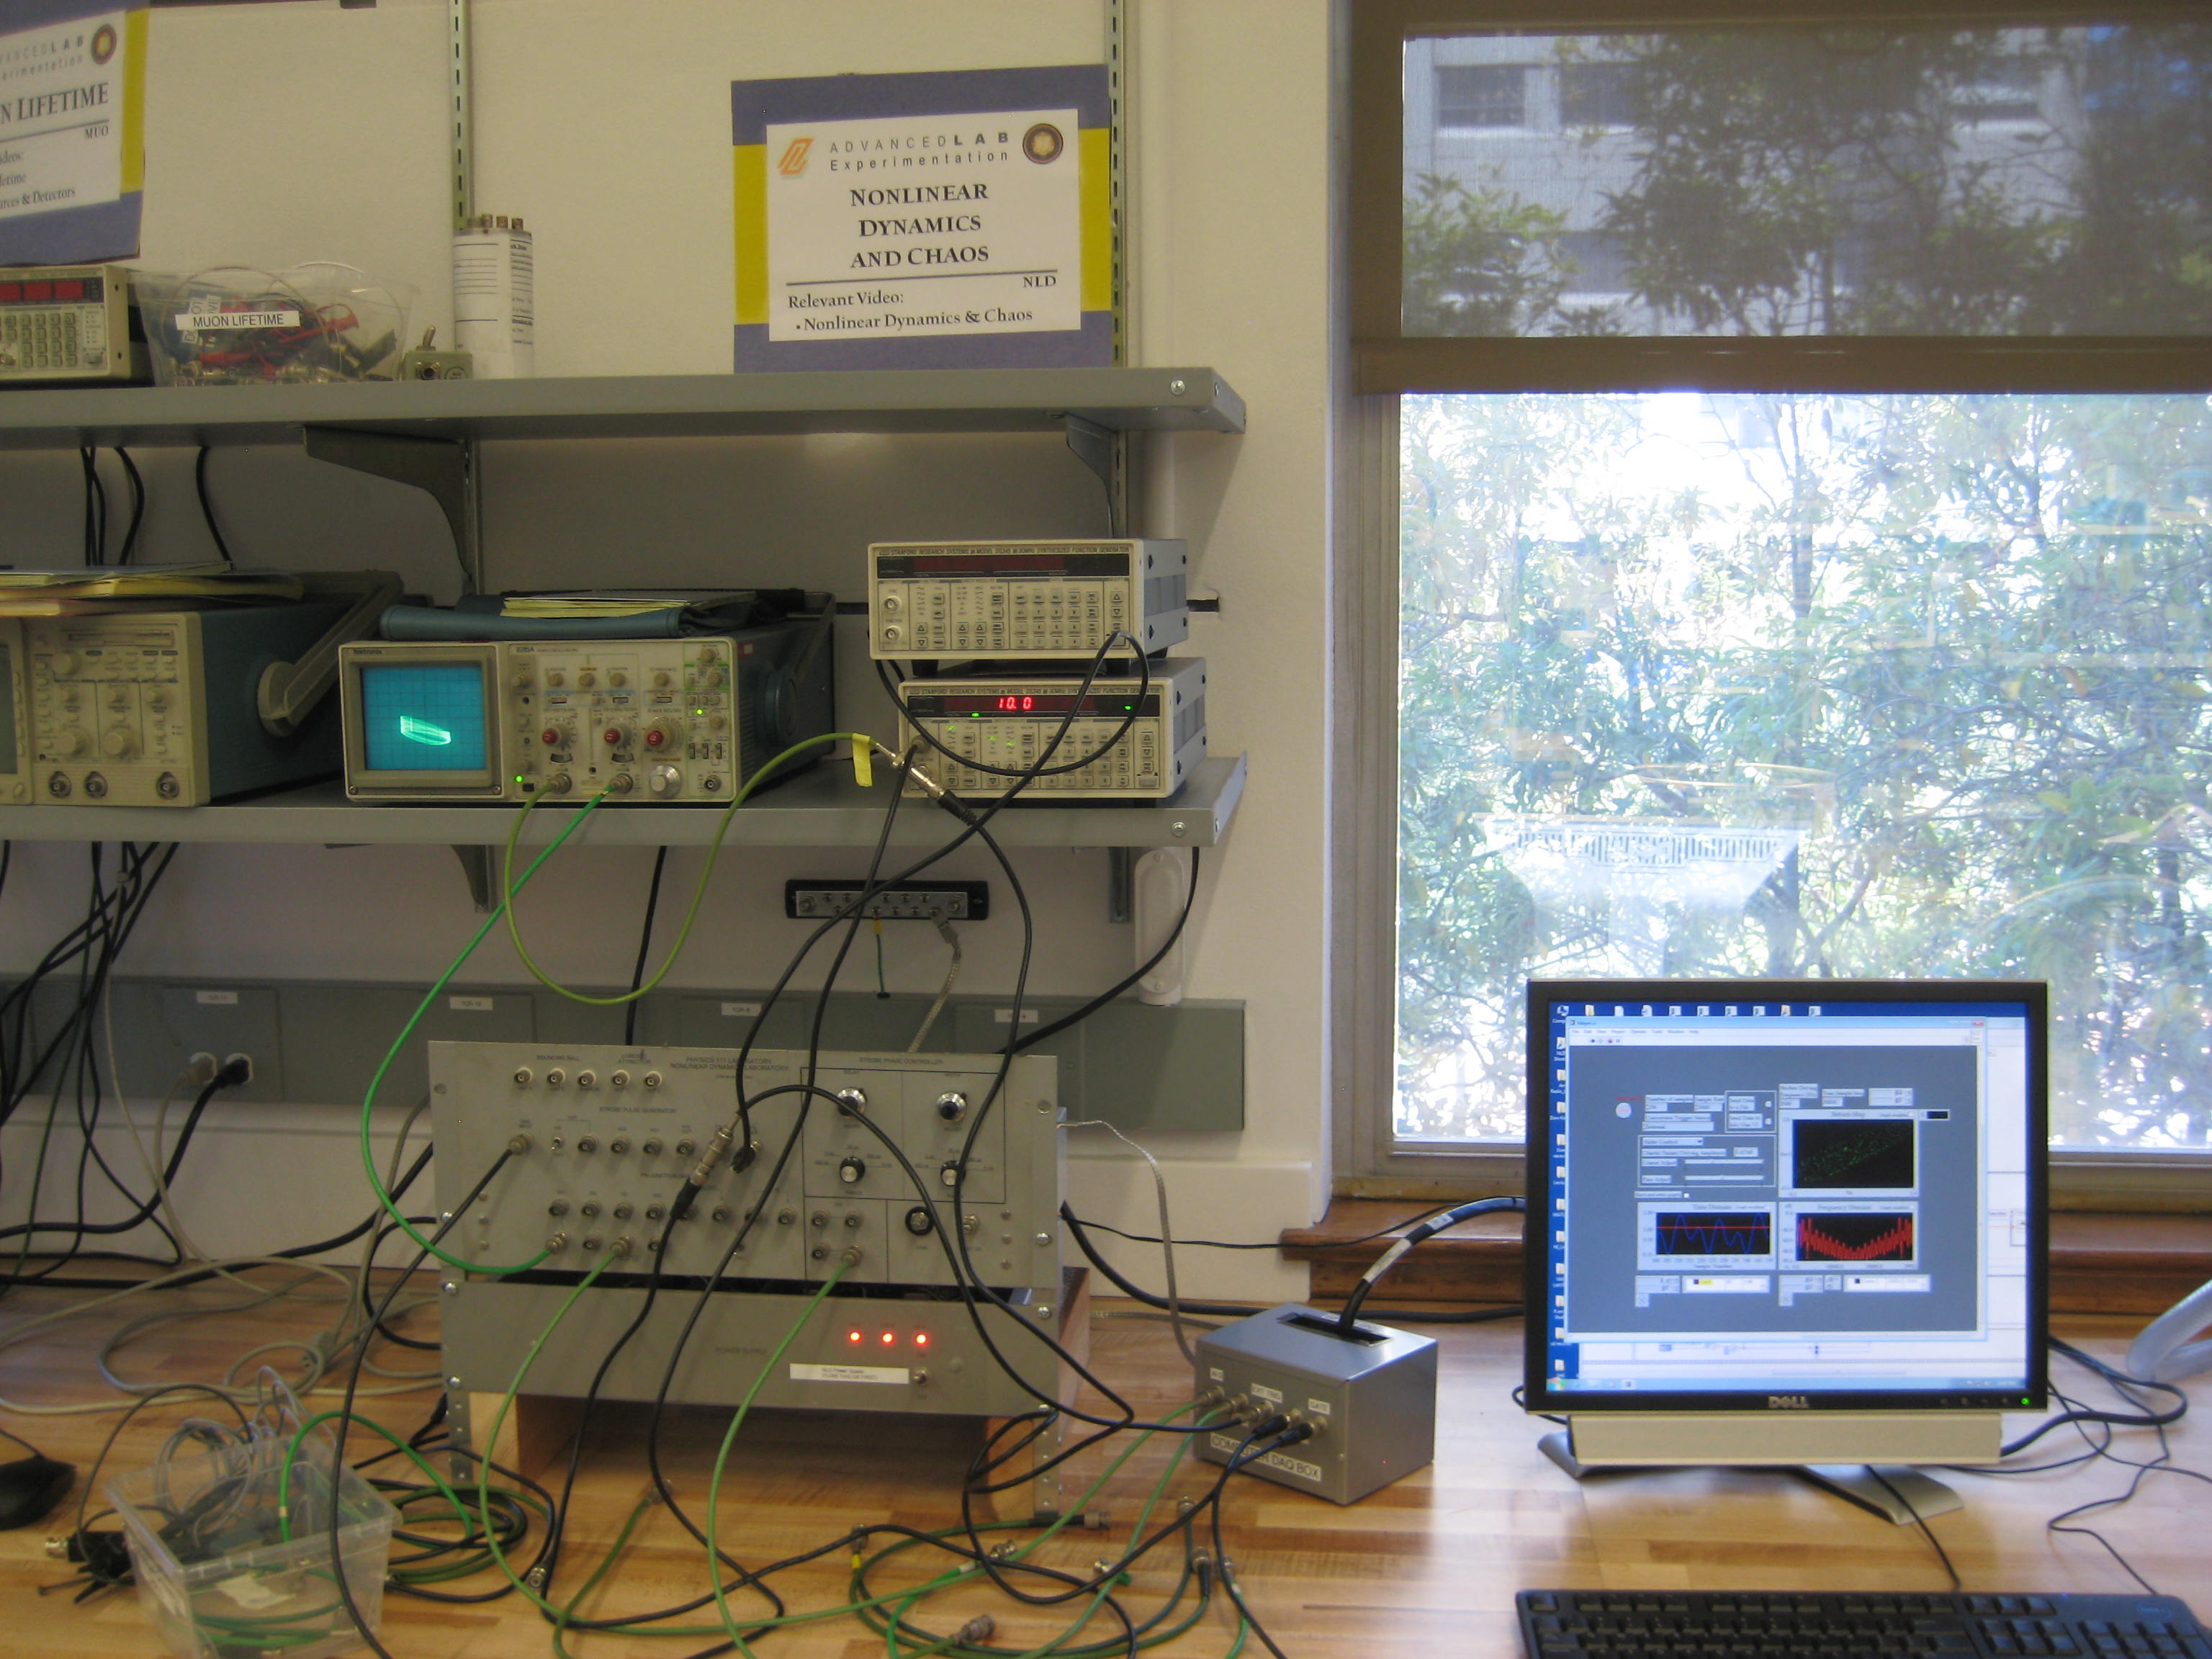
\includegraphics[width=0.7\linewidth]{images/NLD_3516.jpg}}
    \caption{The NLD Chaos Experiment. See larger image \href{http://experimentationlab.berkeley.edu/sites/default/files/images/NLD_3516.jpg}{\textbf{here}}}
\end{figure}

\section{Reading Materials}

\emph{\textbf{Suggested Initial Reading}}: Ref.~\cite{Strogatz}; Skim \S1, \S2.0-\S2.2, \S3.0-\S3.4, \S3.6, and then read \S9.0, \S9.2-9.4, \S10.1-\S10.5 (\S10.6, \S10.7 optional), \S11, \S12.0-\S12.3

\begingroup
\renewcommand{\addcontentsline}[3]{}%
\renewcommand{\section}[2]{}%
\begin{thebibliography}{}
    \bibitem{Strogatz} S. H. Strogatz, \href{http://physics111.lib.berkeley.edu/Physics111/Reprints/NLD/Strogatz_Nonlinear_dynamics_n_chaos.pdf}{\textbf{Nonlinear Dynamics and Chaos}}, (Addison-Wesley, New York, 1994). \#Q172.5.C45 S767\emph{This is an introductory book presuming no prior familiarity with the subject.}

    \bibitem{Ott} E. Ott, \href{http://experimentationlab.berkeley.edu/sites/default/files/chaosindynamicalsystems.pdf}{\textbf{Chaos in Dynamical Systems,}} (Cambridge University Press, 1993). \#Q172.5.C45O87\emph{An excellent, broad, introductory book for advanced students.}

    \bibitem{Schuster} H. G. Schuster, \emph{\href{http://physics111.lib.berkeley.edu/Physics111/Reprints/NLD/13-Shannons\_Measure\_of\_Information.pdf}{\textbf{Deterministic Chaos, an Introduction}}} 2nd ed. (VCH New York, 1988). \#QC174.84.S381\emph{An introductory book appropriate for those with an advanced mathematical background.}

    \bibitem{Press} W. H. Press et al., \emph{\href{http://physics111.lib.berkeley.edu/Physics111/Reprints/NLD/11-Fourier\_Transform\_Spectral\_Methods.pdf}{\textbf{Numerical Recipes in C}}} (Oxford University Press, New York, 1988). \#QA76.73C15 N865\emph{A compendium of numerical algorithms for all branches of science. It is included here for its discussion of the Fourier transform algorithm.}

    \bibitem{Zimmerman} R. L. Zimmerman et al., ``\href{http://ajp.aapt.org/resource/1/ajpias/v60/i4/p370\_s1}{\textbf{The electronic bouncing ball}},'' Am. J. Phys. \textbf{60}, 370 (1992). \href{http://physics111.lib.berkeley.edu/Physics111/Reprints/NLD/14-Electronic\_Bouncing\_Ball.pdf}{\textbf{Searchable Page}}

    \bibitem{Kadanoff} Leo P. Kadanoff, ``\href{http://physics111.lib.berkeley.edu/Physics111/Reprints/NLD/01-Chaos-A\_View\_of\_Complexity.pdf}{\textbf{Chaos: A View of Complexity in the Physical Sciences}}'', Encyclopedia Britannica(1986), pp. 63-92.\emph{Excellent brief introduction.}

    \bibitem{Hao} Bai-Lin Hao. ``\href{http://physics111.lib.berkeley.edu/Physics111/Reprints/NLD/02-Chaos.pdf}{\textbf{Chaos}}'', World Scientific Publishers, Singapore, 1985.\emph{General introduction with reprints of papers in this field.}

    \bibitem{Cvitanovic} P. Cvitanovic, ``\href{http://physics111.lib.berkeley.edu/Physics111/Reprints/NLD/03-Universality\_in\_Chaos.pdf}{\textbf{Universality in Chaos}}'', Acta Physica Dolonica \textbf{A65}, 203-239 (1984).

    \bibitem{Buskirk} R. Van Buskirk and C. D. Jeffries, ``\href{http://link.aps.org/doi/10.1103/PhysRevA.31.3332}{\textbf{Observation of chaotic dynamics of coupled nonlinear oscillators}}'', Phys. Rev. A \textbf{31}, 3332 (1985). \emph{A description of a driven on junction resonator, similar to that of the laboratory experiment.} \href{http://physics111.lib.berkeley.edu/Physics111/Reprints/NLD/09-Observation\_of\_Chaotic\_Dynamics.pdf}{\textbf{Searchable Page}}

    \bibitem{Henon} M. Henon, ``\href{http://projecteuclid.org/DPubS?verb=Display&version=1.0&service=UI&handle=euclid.cmp/1103900150&page=record}{\textbf{A Two-Dimensional Mapping with a Strange Attractor}}'',Comm. Math. Phys. \textbf{50}, 69-77 (1976).\emph{Introduction of the Hènon map; fractal strucure.} \href{http://physics111.lib.berkeley.edu/Physics111/Reprints/NLD/06-A\_Two-Dimensional\_Mapping.pdf}{\textbf{Searchable Page}}

    \bibitem{Feigenbaum} M. Feigenbaum, ``\href{http://physics111.lib.berkeley.edu/Physics111/Reprints/NLD/05-Universal_Behavior.pdf}{\textbf{Universal Behavior in Nonlinear Systems}}'', Physica \textbf{7D}, 16-39 (1983).\emph{Introduction to universality; the quadratic map.}

    \bibitem{Bracewell} R. N. Bracewell, ``\href{http://physics111.lib.berkeley.edu/Physics111/Reprints/NLD/07-The\_Discrete\_Fourier\_Transform.pdf}{\textbf{The Discrete Fourier Transform}}'', ch.18-The Fourier Transform and its Applications, 2nd edition, McGraw Hill (1978).\emph{Brief Introduction to the fast Fourier Transform.}

    \bibitem{Testa} J. Testa, J. Perez, C. Jeffries, ``\href{http://prl.aps.org/abstract/PRL/v48/i11/p714\_1}{\textbf{Evidence for Universal Chaotic Behavior of a Driven Nonlinear Oscillator}}'', Phys. Rev. Lett. \textbf{48}, 714-717 (1982).\emph{Experimental results on the driven pn junction; essentially the experimental system used in the Physics 111-Lab Experiment.} \href{http://physics111.lib.berkeley.edu/Physics111/Reprints/NLD/08-Evidence\_for\_Universal\_Chaotic\_Behavior.pdf}{\textbf{Searchable Page}}

    \bibitem{Theiler} J. Theiler, ``\href{http://www.opticsinfobase.org/abstract.cfm?uri=josaa-7-6-1055}{\textbf{Estimating fractal dimension}},'' J. Opt. Soc. Am. A \textbf{7}, 1055 (1990).\emph{Another review article with an excellent bibliography. This one focuses on fractals. } \href{http://physics111.lib.berkeley.edu/Physics111/Reprints/NLD/16-Estimating\_Fractal\_Dimension.pdf}{\textbf{Searchable Page}}

    \bibitem{Abarbanel} Abarbanel, ``Making Physics From Chaos,'' videotape, \#QA845 A77, on reserve in the physics library.\emph{An application of NLD to turbulence around torpedoes. The talk is clear but the speaker runs out of time.}

    \bibitem{Clark} B. K. Clark et al., ``\href{http://ajp.aapt.org/resource/1/ajpias/v63/i2/p157\_s1}{\textbf{Fractal dimension of the strange attractor of the bouncing ball circuit}},'' Am. J. Phys. \textbf{63}, 157 (1995).\href{http://physics111.lib.berkeley.edu/Physics111/Reprints/NLD/15-Fractal\_Dimension.pdf}{\textbf{Searchable Page}}

    \bibitem{Shannon} C. E. Shannon, \href{http://experimentationlab.berkeley.edu/sites/default/files/mathematicaltheorycommunication.pdf}{\textbf{The mathematical theory of communication}}, (University of Illinois Press, Urbana, 1964). \#TK5101 .S45

    \bibitem{May} R. May, ``\href{http://www.nature.com/nature/journal/v261/n5560/abs/261459a0.html}{\textbf{Simple Mathematical Models with very Complicated Dynamics}}'' Nature \textbf{261}, 459-467 (1975).\emph{Important early review of nonlinear maps.}\href{http://physics111.lib.berkeley.edu/Physics111/Reprints/NLD/04-Simple\_Mathematical\_Models.pdf}{\textbf{Searchable Page}}

    \bibitem{Perez} J. Perez, and C. Jeffries, ``\href{http://prb.aps.org/abstract/PRB/v26/i6/p3460\_1}{\textbf{Effects of additive noise on a nonlinear oscillator exhibiting period doubling and chaotic behavior}}'', Phys. Rev. B \textbf{26}, 3460-3462 (1982).\emph{Experiment results on adding noise to the driven on junction.} \href{http://physics111.lib.berkeley.edu/Physics111/Reprints/NLD/10-Effects\_of\_Additive\_Noise.pdf}{\textbf{Searchable Page}}

    \bibitem{Hamming} R. W. Hamming, ``\href{http://physics111.lib.berkeley.edu/Physics111/Reprints/NLD/12-Maximum\_Entropy.pdf}{\textbf{Maximum Entropy}}'', The Art of Probability for Scientists and Engineers: Chp.7, pp. 253-265 + 7 pages of diagrams

    \bibitem{Eckmann} J. P. Eckmann, and D. Ruelle. ``\href{http://rmp.aps.org/abstract/RMP/v57/i3/p617\_1}{\textbf{Ergodic Theory of Chaos and Strange Attractors}}'', Rev. Mod. Phys. \textbf{57}, 617-656 (1985). \href{http://physics111.lib.berkeley.edu/Physics111/Reprints/NLD/17-Ergodic\_Theory.pdf}{\textbf{Searchable Page}}

    \bibitem{Wells} L. Wells and J. Travis \emph{LabVIEW for Everyone, }Prentice Hall PTR (Available from Don Orlando).
\end{thebibliography}
\endgroup

Reprints and reference materials can be found on the \href{http://physics111.lib.berkeley.edu/Physics111/Reprints/NLD/NLD\_index.html}{\textbf{Physics 111 Library Site}}

\section{Objectives}

\begin{itemize}
    \item Learn what real experimental physics is about

    \item Learn the synergy between experimental and theoretical work

    \item Learn to use pieces of equipment that are commonly used in research

    \item Learn how measurements are performed, analyzed, and interpreted.

    \item Learn how to present your work and results

    \item Learn problem solving strategies

    \item Learn how to manage and organize your time
\end{itemize}

\section{Introduction}

This experiment is an introduction to Non-Linear Dynamics, Data Acquisition, Chaos theory and Fractals. Limited as we are by our senses and relatively short powers of recall, much of the physical world seems aperiodic and defies quantitative description. While we have yet to discover closed form solutions to the simplest of systems (e.g. the one-dimensional gravitational three-body problem), the field of chaos reveals structure in their dynamics. The results of chaos theory have found practical applications in almost every branch of science.

The term Chaotic has come to mean something very specific in this field. It does not mean random or unorganized as the ordinary English word does. It refers instead to a particular type of dynamical behavior. One which at first sight appears random, but underlying it are ordered deterministic laws. Chaotic systems exhibit these key features: They are aperiodic, they exhibit sensitive dependence on initial conditions, and they are in some sense bounded.

\section{Equipment used in this experiment}

\begin{enumerate}
    \item Function Signal Generator \href{https://youtu.be/PrM8DHFOFS0}{\textbf{SRS DS 345}}

    \item Computer interface Box

    \item DAQ card in computer

    \item Main Control Chassis NLD-86-35Rev2002

    \item Bouncing Ball and Lorenz Attractor inside control chassis

    \item Scope

    \item Power Supply providing +15/$-$15/+5 V

    \item Rack for equipment
\end{enumerate}

\section{Theory}

\subsection{The PN Junction: An Introductory Dynamical System}

A \emph{dynamical system} is essentially anything that varies with time. The pertinent variables necessary to describe its motion are called the \emph{dynamical variables} and the evolution of the system describes a path, or \emph{trajectory} in the \emph{state-space} (also called \emph{phase space}) of the dynamical variables. Dynamical systems may be either \emph{conservative}: a volume element in state space remains invariant (recall Liouville's theorem; see Marion, J. B. \emph{Classical dynamics of particles \& systems}); or the system may be \emph{dissipative}: for which regions of state space become compressed as the systems evolves.

One of the dynamical systems we study is a driven damped oscillator with a non-linear response. Because it is damped this is a dissipative system. It consists of a pn-junction (a diode) connected in series with an inductor L, a resistor R, and a driving sine wave oscillator of voltage $V_0(t) = V_{os} \cos(\omega_0 t) $, see the left side of Figure \ref{fig:Circuit}.

\begin{figure}[h]
    \centering
    \href{http://experimentationlab.berkeley.edu/sites/default/files/images/Nldimage004.gif}{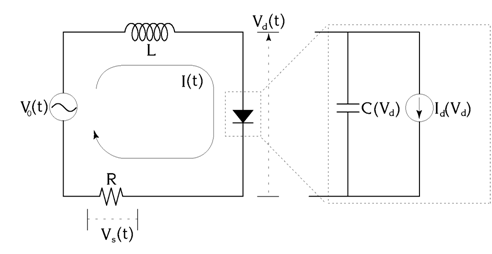
\includegraphics[width=0.5\linewidth]{images/Nldimage004.png}}
    \caption{Driven damped oscillator circuit with a closeup of the diode.}
    \label{fig:Circuit}
\end{figure}

\begin{figure}[h]
    \centering
    \href{http://experimentationlab.berkeley.edu/sites/default/files/images/Nldimage005.gif}{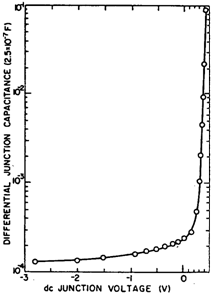
\includegraphics[width=0.4\linewidth]{images/Nldimage005.png}}
    \caption{Capacitance of a typical diode as a function of diode voltage. From Ref. \cite{Hao}.}
    \label{fig:CapacitanceOfTypicalDiode}
\end{figure}

The diode is the non-linear circuit element: not only does it have an exponential $I$-$V$ characteristic,

\begin{equation}
    I_d(V_d) = I_0[\exp(eV_d / kT) - 1]
\end{equation}

but due to the properties of the junction (see Ref. \cite{Cvitanovic}), it has a non-linear capacitance as well. The capacitance may be written as a function of the voltage across the diode, \emph{$V_{d}$}:

\begin{equation}
    C(V_d) =
    \begin{cases}
        C_0 e^{eV_d/kT} &: V_d > 0 \\
        \frac{C_0}{\sqrt {1-e^{eV_d/kT}}} &: V_d \le 0
    \end{cases}
\end{equation}
 
Thus the diode may be modeled as a voltage-dependent capacitor connected in parallel with an ideal diode (a voltage-dependent current-source), giving the equivalent circuit on the right of Figure 1.

We use a computer to measure the voltage across the resistor $R$ and the observed signal, $V_s(t)$, is proportional to the current $I(t)$.

For small values of driving voltage, the diode doesn't conduct, its capacitance is nearly constant, and the circuit behaves like a passive LRC resonator: A standard treatment of which yields a resonant frequency $\omega_\text{res} \approx 1/\sqrt{LC( V_d = 0)} = 1/\sqrt{LC_0}$. But as the driving amplitude increases, the increasing diode capacitance drops the resonant frequency significantly.

The effect of increasing driving-amplitude is seen in the following figures. They are plots of $I(t)$ (measured as $Vs(t)$ in Volts) vs. time (measured in sample number of a 50 kHz clock). In all three plots the driving oscillator is operating at the same frequency, $\omega_\text{res} \approx$ 3.5 kHz (a period of $\approx$ 15 samples).

\begin{figure}[h]
\begin{minipage}{0.32\textwidth}
    \href{http://experimentationlab.berkeley.edu/sites/default/files/images/Nldimage014.gif}{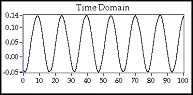
\includegraphics[width=\linewidth,keepaspectratio]{images/Nldimage014.png}}
    \caption{$I(t)$. $V_{os} \approx$ 0.3 V, response period $\approx$ 15 samples.}
    \label{fig:Period15}
\end{minipage}\hfill
\begin{minipage}{0.32\textwidth}
    \href{http://experimentationlab.berkeley.edu/sites/default/files/images/Nldimage015.jpg}{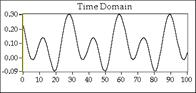
\includegraphics[width=\linewidth,keepaspectratio]{images/Nldimage015.jpg}}
    \caption{$I(t)$. $V_{os} \approx$ 0.5 V, response period $\approx$ 30 samples.}
    \label{fig:Period30}
\end{minipage}\hfill
\begin{minipage}{0.32\textwidth}
    \href{http://experimentationlab.berkeley.edu/sites/default/files/images/Nldimage016.jpg}{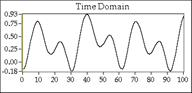
\includegraphics[width=\linewidth,keepaspectratio]{images/Nldimage016.jpg}}
    \caption{$I(t)$. $V_{os} \approx$ 1.5 V, response period $\approx$ 60 samples}
    \label{fig:Period60}
\end{minipage}
\end{figure}

In Figure \ref{fig:Period15}, $V_{os}$ is set to a small value and the response signal $V_s(t)$ is a sine wave; this is the linear response. As $V_{os}(t)$ is increased, $V_s(t)$ begins to produce harmonic content at 2$\omega_0$, 3$\omega_0$ etc (not shown). But as you keep increasing the voltage, it will abruptly exhibit a change in behavior that, for reasons that will become clearer later, is called a \emph{bifurcation}. This new state has \emph{sub}harmonic content $\omega_0/2$ (Figure \ref{fig:Period30}) and consequently is also called a \emph{period-doubling} bifurcation. As $V_{os}$ is further increased, this period doubling bifurcation occurs again and again at increasingly closely spaced values of $V_{os}$. As the period approaches infinity, the system becomes \emph{chaotic}, i.e. it is aperiodic, with a small but visible noise-like component that looks like ``jitter.''

\begin{figure}[h]
    \centering
    \href{http://experimentationlab.berkeley.edu/sites/default/files/images/Nldimage019.jpg}{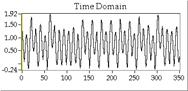
\includegraphics[width=0.5\linewidth]{images/Nldimage019.jpg}}
    \caption{$I(t)$. $V_{os} \approx$ 3.5 V. The diode response current is now aperiodic.}
    \label{fig:Nldimage019}
\end{figure}

As $V_{os}$ is further increased, this ``noise'' dominates the trace; however, one finds narrow ranges of $V_{os}$ (``windows'') for which this noise completely disappears, leaving a periodic signal. This noise is not random noise due to fluctuation phenomena (e.g., Johnson noise, shot noise, flicker noise), but is a natural consequence of the non-linear equations of motion of the system. As such, it is determined by the solution of the equations. We call this noise chaos. When the system becomes chaotic, Fourier spectral analysis shows a transition from a discrete to a continuous distribution.

The above behavior, a period-doubling cascade to chaos, is observed in many physical, chemical, and biological systems. To better understand it we shift our attention from the time domain to state-space.

The equations (of motion) for the PN-junction (Ref.~\cite{Cvitanovic}, Sec. II) are:
\begin{align}
    \label{eq:Motion1}
    \dot I &= \frac{V_0 - RI - V_d}{L} \\
    \label{eq:Motion2}
    \dot V_d &= \frac{I - I_d(V_d)}{C(V_d)} \\
    \label{eq:Motion3}
    \dot \theta &= \omega \text{ (the time derivative of the driving signal's phase)}
\end{align}
Notice that these equations do not depend explicitly on time (and so are called \emph{autonomous}). Instead they relate the rate of change of the current state to the current state itself. That is, given a state-space $M$ of the variables ($I$, $V_d$, $\theta$), we may write equations \eqref{eq:Motion1}-\eqref{eq:Motion3} as one vector equation
\begin{equation}
    \dot{\vec p} = \vec F (\vec p) \text{ where }p \in M
\end{equation}
Thus $\vec p$ denotes the current state of the system, and $\vec p(t)$ the path of the system through the three-dimensional state-space of the dynamical variables.

\subsection{Phase-Path Reconstruction}

If one could measure all the dynamical variables of a system simultaneously, the path $\vec p(t)$ could be plotted easily. However, in many cases this is not possible and, moreover, it is not necessary in most cases. Look ahead to the reconstructed phase plots of Figures 7 to 10. These plots were made by sampling the diode current only. Rather than measuring the complete set of variables $(I, V_d, \theta)$, the trajectory is available in \emph{each} variable (i.e. we could have sampled the diode voltage and come up with similar plots).

Sampling only one dynamical variable and reconstructing the trajectory in a higher-dimensional space is a process called \emph{embedding}: Given a \textbf{discrete time series} $\{I_n\} $ of regularly sampled values of $I_d(t_0 + n\tau)$, where $t_0$ is an arbitrary initial time and $\tau$ is the sample period, we embed the current in a higher dimension (appropriately called the \emph{embedding-dimension,} in this example, dimension 3) by forming the points $(I_n, I_{n+1}, I_{n+2})$ for all data.

This set of points then reveals an object topologically equivalent to the actual path in state-space. That this works is rather surprising. Ott presents a precise explanation (Ref.~\cite{Ott}, section 3.8), but the basic idea is that if you know the current at a given moment, $I_n$ that information gives you a little bit of information about where you are in state-space, that is, any point where the plane $I = I_n$ intersects all possible trajectories. You then refine your knowledge by stipulating that you're at the point where not only is the current $I_n$ but the current was $I_{n-1}$ at a time $\tau$ in the past. This pins down the location further, and subsequent restrictions on what the current was in the past refines your knowledge about what state it's in now.

This is by no means obvious, and it's complicated by the fact that there do exist situations where it doesn't work. But that the geometric properties of the system's trajectory can be found by sampling only one of the state-variables is remarkable and useful: It means that the structure of large-scale, multi-dimensional dynamical systems is available to a simple, single-detector apparatus.

\subsection{PN-Junction phase plots \& The Bifurcation Route to Chaos}

Figure 7- Figure 10 show reconstructed phase-space trajectories, $ \vec p(t) $, that correspond to the circuit's operation in Figure 3- Figure 6. The plots were made using the embedding technique described in the previous section, so the plot axes are $ (I_n, I_{n+1}, I_{n+2}) $. We speculate that $\theta$ revolves around the line $z = y = x$, and that the other two state variables, V and I, correspond loosely to the distance along that line and the distance from that line. The graphs are all stereo-optic. Try holding them at arm's length (or set them on a desk as you stand over them) and letting your eyes focus at infinity. Let two of the double images overlap so that you can see three images. The middle one, if you get it to match up just right, will look like it's 3D.

\begin{figure}
    \centering
    \href{http://experimentationlab.berkeley.edu/sites/default/files/images/Nldimage042.gif}{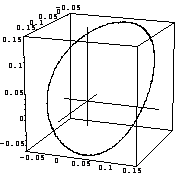
\includegraphics[width=0.33\linewidth,keepaspectratio]{images/Nldimage042.png}}
    \href{http://experimentationlab.berkeley.edu/sites/default/files/images/Nldimage043.gif}{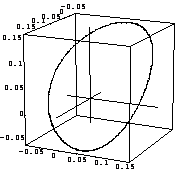
\includegraphics[width=0.33\linewidth,keepaspectratio]{images/Nldimage043.png}}
    \caption{Left and Right stereo-optic images of the linear response of the PN-Junction. The path is almost an ellipse, which is the path of a simple harmonic oscillator.}
    \label{fig:my_label}
\end{figure}

\newpage

For small values of the parameter $V_{os}$, the trajectory is a stable orbit. For larger value (after bifurcation to period 2) the orbit is still stable, but requires \emph{two} cycles of the driving oscillator to return to its initial point (Figure 8). These trajectories are a subclass of a more general object called an \emph{\textbf{attractor}}: The subset of state space toward which a dynamical system evolves. Because they are periodic (the paths are closed cycles), the simple attractors of Figure 7-Figure 9 are known as \emph{\textbf{limit-cycles}}.

\begin{figure}
    \centering
    \href{http://experimentationlab.berkeley.edu/sites/default/files/images/Nldimage044.gif}{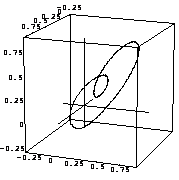
\includegraphics[width=0.33\linewidth,keepaspectratio]{images/Nldimage044.png}}
    \href{http://experimentationlab.berkeley.edu/sites/default/files/images/Nldimage045.gif}{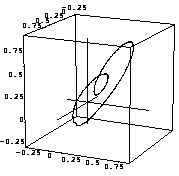
\includegraphics[width=0.33\linewidth,keepaspectratio]{images/Nldimage045.png}}
    \caption{L \& R images of the diode response after undergoing a period-doubling bifurcation}
\end{figure}

\begin{figure}
    \centering
    \href{http://experimentationlab.berkeley.edu/sites/default/files/images/Nldimage046.gif}{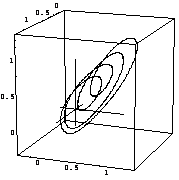
\includegraphics[width=0.33\linewidth,keepaspectratio]{images/Nldimage046.png}}
    \href{http://experimentationlab.berkeley.edu/sites/default/files/images/Nldimage047.gif}{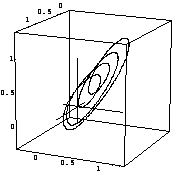
\includegraphics[width=0.33\linewidth,keepaspectratio]{images/Nldimage047.png}}
    \caption{Same as above after another bifurcation.}
\end{figure}

Increasing $V_{os}$ to the point where the system is chaotic reveals a more complicated attractor: it is a \emph{\textbf{fractal}} object and hence called a \emph{\textbf{strange}} attractor.

\begin{figure}
    \centering
    \href{http://experimentationlab.berkeley.edu/sites/default/files/images/Nldimage048.gif}{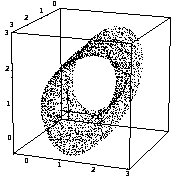
\includegraphics[width=0.33\linewidth,keepaspectratio]{images/Nldimage048.png}}
    \href{http://experimentationlab.berkeley.edu/sites/default/files/images/Nldimage049.gif}{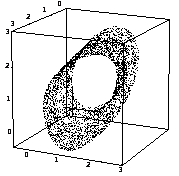
\includegraphics[width=0.33\linewidth,keepaspectratio]{images/Nldimage049.png}}
    \caption{The system is now chaotic. The path in phase space never closes. And the evolution traces out the system's attractor. To improve the visibility of the plot the lines connecting the points have been omitted.}
\end{figure}

\subsection{Fractals}

As you learned in calculus, most geometrical objects become smoother as one gets closer and closer to them. Fractals, however, remain twisty and crumpled no matter how close one scrutinizes them. As such, they defy conventional definitions of length and volume. Efforts to quantify fractals first led to several different definitions of dimension and finally to generalized dimension (Ref.~\cite{Schuster}, Section 5.3, Ref.~\cite{Press} p1060, Ref.~\cite{Ott}, p78), the most intuitive of which is:

\[
    \text{bulk} \propto \text{size}^\text{dimension}, \text{so that }  \text{dimension} = \lim_{\text{size} \to 0} \frac{\ln \text{bulk}}{\ln \text{size}}
\]
for appropriate definitions of bulk and size. Note that taking the limit as size $\to$ 0 means that this definition of dimension is a local property of the object and may vary over its extent.

For instance, in two dimensions a disk has an Area $\propto$ radius$^2$, and $\lim_{r \to 0}\frac{\ln\pi r^2}{\ln r} = 2$. With this definition, objects of non-integral dimension are called fractals.

\subsection{Flow and Liapunov Exponents}

Chaotic systems are noted for several universal features: The bifurcation route to chaos; Stable windows of periodicity, the borders of which exhibit short bursts of chaotic signal (``intermittency''); And sensitivity to initial conditions. To help explain some of these features, we define a \emph{\textbf{flow}} $ \phi_t $ that maps a state $ \vec p $ to its new state $ {\phi}_t(\vec p) $ at a time \emph{t} units later. This operation also satisfies the relationship:
\[
    \phi_t(\phi_s(\vec p)) = \phi_{t+s}(\vec p)
\]
Now consider two neighboring initial conditions $\vec P_0 \text{ and } \vec P_0+\vec h$. Expanding $\phi_t(\vec P_0+\vec h)$ about $\vec P_0$ gives $\phi_t(\vec P_0+\vec h) = \phi_t(\vec P_0) + \bar{\bar J}(t)\vec h + O(\| h\|^2) + \ldots$ where $\bar{\bar J}(t)$ is the Jacobian matrix of partial derivatives of $\phi_t$ with respect to $\vec P_0$ and $O(\| h\|^2) + \ldots$ are higher order terms. (In one dimension, $\bar{\bar J}(t)$ would just be $ \frac{\partial\phi}{\partial x}(t) $). Thus we see that a small displacement in initial conditions $ \vec h $ is magnified to $ \bar{\bar J}(t)\vec h $. The evolution of the distance between neighboring initial-conditions is then given by the eigenvalues of $ \bar{\bar J}(t) $. \emph{Liapunov} (alternately spelled Lyapunov or Ljapunov) \emph{exponents} are convenient measures of the eigenvalues and are defined as
\begin{equation}
    \lambda_n \equiv \lim_{t \to \infty}\frac{\ln| n^\text{th} \text{ eigenvalue of } \bar{\bar J}| }{t}
\end{equation}
If the Liapunov exponents are all positive then the system diverges. If they are all negative then the system condenses to a point. If the largest one is positive and the sum of them all is negative, then it amounts to a stretch in one or more dimensions and a contraction in the others and chaotic behavior is guaranteed.

\subsection{Recurrence relations}

\newpage

The equations of state (Eq's \eqref{eq:Motion1}, \eqref{eq:Motion2}, 
\eqref{eq:Motion3}) are functions of a continuous time variable. Using the Runge-Kutta method of integrating ordinary differential equations, it is possible to form a set of discrete-time dynamical equations and these are seen to exhibit universal features common to other similar systems. For this reason, we study \emph{\textbf{iterative maps}}: discrete versions of $ \phi_t $ that relate the next state of a system to its previous state. You might wonder why, if chaotic systems are so sensitive to initial conditions, should we expect to see any useful results computed by an approximating method such as Runge-Kutta. The reason is explained in [Ref.~\cite{Strogatz}, \S10.1], where the authors present the 'shadowing' lemma: Although a finitely computed chaotic time-series, beginning with an initial value, will rapidly diverge from the true orbit, there exists some other orbit that coincides closely to the computed series.

\section{The Experiment Apparatus}

This experiment uses an Intel CPU based computer, running the Windows operating system. The main tools are a data-acquisition computer-interface card and the LabView software package. The data-acquisition card has 8 input-channels, 2 output channels, and miscellaneous timing and TTL features. The inputs sample voltages in the ±5 Volt range with 12-bit resolution at speeds to 100khz.

LabView is a graphical programming environment designed to facilitate lab-instrument control, data-acquisition, and rudimentary numerical analysis. There is a suite of LabView programs (called VI's; for Virtual Instruments) specifically written for this lab that constitutes the bulk of this experiment. You'll also be writing a few of your own to get a better feel for LabView.

Most of the non-linear circuits you will examine in this lab are driven, so the computer is set up to modify a driving voltage, by using its DAC to attenuate a function-generator, and measure the circuit's response (see Figure~\ref{fig:SimplifiedBlockDiagram}). Because you won't be starting with the real systems, the details of the equipment and connections are deferred to section 4.5, where they should make more sense.

\begin{figure}[h]
    \centering
    \href{http://experimentationlab.berkeley.edu/sites/default/files/images/Nldimage066.gif}{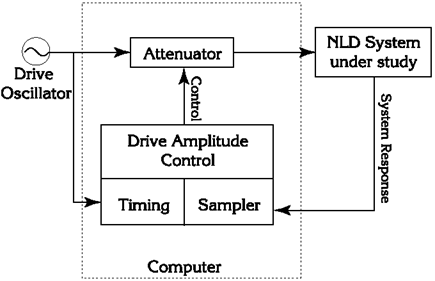
\includegraphics[width=0.7\linewidth]{images/Nldimage066.png}}
    \caption{Simplified block diagram.}
    \label{fig:SimplifiedBlockDiagram}
\end{figure}

\section{Procedures}

\subsection{Getting started with LabView and Sampling}

Before starting LabView, create a directory for yourself inside My Documents folder. This is where you will save ALL your work. Read chapters 1-3 in LabView for Everyone and be sure to do the exercises. If you know LabView from BSC then proceed. Otherwise this will help immensely, especially if you have no previous programming experience. Here is a list of helpful things you might want to know:

\begin{itemize}
    \item Control-H displays ``pop-up'' help, which will automatically explain things you point to with your cursor. Usually, this is sufficient, but if you need more detailed information, use the LabView manuals provided with the experiment.

    \item Control-E switches between the \emph{front-panel} and the \emph{diagram} windows.

    \item There are 3 palettes you will be using; \emph{functions}, \emph{controls}, and \emph{tools}. Right clicking the mouse brings the appropriate palette for the window you're working in. \emph{Functions }are used in the diagram window, \emph{controls }are used\emph{ }in the front-panel window, and \emph{tools} are used in both. Use the spacebar to switch between different tools in the \emph{tools }palette.

    \item The LabView modules/elements (the things that look like icons) are unique in that there aren't two of them that look the same but do different things. Thus if your diagram looks just like the one in the lab manual, it will probably do the same thing.

    \item If you can't find an element/module, you may have to pick a similar one and then modify it.

    \item Wire from the input devices towards the output. Sometimes, the type of input to a module affects the output.

    \item Placing objects in the \emph{front-panel} window places corresponding objects in the \emph{diagram} window. It's a good idea to make the \emph{front-panel} first, as then all of the corresponding objects are in place and you can plan what to do with them.

    \item Objects in the \emph{front-panel} which represent numbers (i.e. slide bars, dials, etc.) or an array of numbers (i.e. charts, graphs) show up in the \emph{diagram} window as [SGL] or [DBL] or [INT] (single or double precision, or integer).

    \item Modules in the \emph{diagram} window have inputs and outputs, and it is important to wire them up correctly. The icon that looks like a spool of wire in the \emph{tools} palette is used for wiring. Placing the mouse cursor over the different areas of the modules will tell you the specific functions of the inputs and outputs. These can sometimes be modified by right-clicking on them with the mouse.

\end{itemize}

Once you're ready to begin, copy all files to your my documents folder chaos. (Note: go to C:\textbackslash support\textbackslash NLD2013 for the NLD.llb file and copy all into your folder manually. Now start LabView from the Windows Start menu. Your first assignment is to make a simple VI. Investigate sampling by putting a \emph{waveform graph} and a \emph{waveform chart} on the front panel. These are located under \textbf{Functions-}F which can be accessed by right clicking in an empty space in ``Block Diagram''.(in the same way the \textbf{Controls} can be accessed by right clicking in an empty space in ``Front Panel''.

\begin{figure}[h]
    \centering
    \href{http://experimentationlab.berkeley.edu/sites/default/files/images/Nldimage067.jpg}{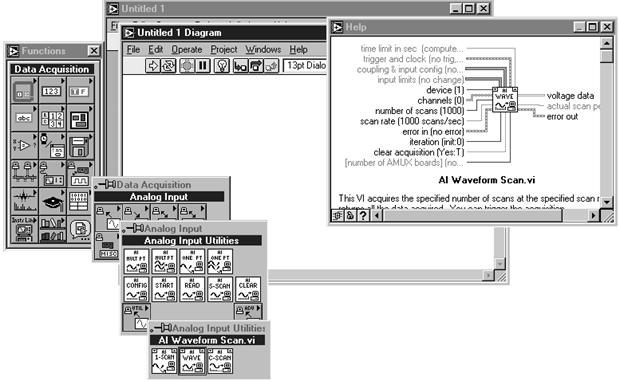
\includegraphics[width=0.5\linewidth]{images/Nldimage067.jpg}}
    \caption{Pop-up help while inserting VI components.}
    \label{fig:Nldimage067}
\end{figure}

\textbf{NOTE: AI Waveform Scan.vi is no more. Everything that requires it is optional. You should be able to find a similar VI in the new LabVIEW.}

Create a VI that reads a signal from the DS345 Function generator using the Computer DAQ box. Here's where to find the modules needed to create your program:

\newpage

\begin{itemize}
    \item Controls $\rightarrow$ Graph Indicators $\rightarrow$ Waveform Chart/Waveform Graph (you will need 2)

    \item Functions $\rightarrow$ All Functions  $\rightarrow$  Measurement I/O  $\rightarrow$  DAQmx $\rightarrow$  DAQ Assist

    \item Functions $\rightarrow$ All Functions $\rightarrow$ Numeric $\rightarrow$ Numeric Constant

    \item Functions $\rightarrow$ All Functions $\rightarrow$ Programming $\rightarrow$ Waveform $\rightarrow$ Analog Waveform $\rightarrow$ Power Spectrum

    \item Functions $\rightarrow$ All Functions $\rightarrow$ NI Measurments $\rightarrow$ Data Acquisition $\rightarrow$ Analog Input $\rightarrow$ Waveform Measurements $\rightarrow$ Spectral Measurements( you can search for this in Labview also)
\end{itemize}

\begin{figure}[h]
    \centering
    \href{http://experimentationlab.berkeley.edu/sites/default/files/NLD/FirstExcersizeBlockDiagram.png}{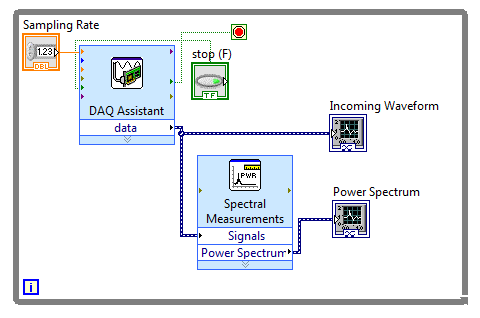
\includegraphics[width=0.5\linewidth]{images/FirstExcersizeBlockDiagram.png}}
    \caption{Connections for the simple sampling VI that you will make.}
    \label{fig:FirstExcersizeBlockDiagram}
\end{figure}

Once you have wired up the VI, you're ready to use it to sample signals. Use a function generator (Stanford Research Systems Model DS345) to send some signal to the Computer DAQ box. Connect the ``function output'' of the function generator to the terminal labeled AI 0 (make sure to terminate the signal). Adjust its output to produce an approximately 200 Hz sine wave, 5 Volts in amplitude (10V peak-to-peak). Use a scope to check the output. Once you create the DAQ Assistant it will prompt you for some inputs, select analog input and then voltage from the ai0 channel. The Spectral measurements one will also prompt you for some information (make sure you program it to spit out the power spectrum in a linear plot).  Run your VI by pressing the ``run'' button.

Your two graphs should display the time-series of the signal (it should look like a sine-wave) and the \emph{discrete} Fourier transform (DFT). We stress that it's the discrete transform because, while it is closely related to the continuous Fourier transform, there are some important differences that we hope you'll discover. The units of the time-series graph are Volts vs. Sample number. What are the units of the DFT window?

The Fourier transform of a sine wave is a delta-function (loosely speaking, a peak). Now change the frequency. Vary it between 100 and 10,000 Hz. See if you can explain what's happening. Also make sure that you are changing the sampling rate on your DAQ Assistant, think about why the sampling rate is important. Is there a way you can confidently predict a sampling rate that will give you an accurate reading of the signal? (Hint: Think back to BSC and the Nyquist criterion)


\textbf{This is a Checkpoint: Call over a professor or GSI and show them your program and explain how it works.  Explain the units on the DFT window, how do read the power spectrum from a time varying signal, and how you were able to accurately sample the incoming signal (explain what frequencies you set when varying the DS345).}

\section{Graphing}

\begin{figure}[h]
    \centering
    \href{http://experimentationlab.berkeley.edu/sites/default/files/images/Nldimage069.gif}{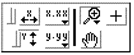
\includegraphics[width=0.3\linewidth]{images/Nldimage069.png}}
    \caption{The graph-axes tool-palette.}
    \label{fig:GraphAxesToolPalette}
\end{figure}

As you experiment with the parameters of the exercise, you may want to change the range of the graphed data. For this purpose, each graph window has its own palette of display controls (Figure~\ref{fig:GraphAxesToolPalette}). These control auto-ranging of the axes, format and precision of the axes, zooming, scrolling and the use of graph markers. See Ch 16 of the LabVIEW User Manual; 2nd Ed.; Jeffrey Travis, for more information. You may also highlight (with the mouse) and type directly onto the axes scales.

Next, change the waveform from a sine to a triangle at 100 Hz. Calculate, or look-up in a reference, the Fourier series of a triangle wave. Does the displayed spectrum match what you expect?1 To help you determine the frequencies of different peaks, you should use graph cursors. You can enable them by right-clicking on the DFT window and selecting ``show?cursor display.'' This displays a palette of controls that permits the marking and measuring of values on the graph. See the LabView manual for details.

The harmonics of the triangle wave that occur above the Nyquist frequency, will be aliased. Adjust the frequency of the function generator between 100 and 800 Hz, and familiarize yourself with the operational details of aliasing.

\subsection{One-dimensional maps: Introductory chaotic systems.}

Multi-dimensional differential equations are hard to study. If they are insoluble, only numerical integration is possible. As simple examples of chaotic systems, one-dimensional maps offer an easy way to explore the defining features of chaos.

To familiarize yourself with 1-d maps, you will write a ``cob-web'' analyzer VI that shows the progress of iterations of the quadratic map (See Figure~\ref{fig:CobWebAnalyzer}). Be sure to at least glance at \S10.2 Ref.~\cite{Strogatz}, to get an idea of what's going on.

\begin{figure}[h]
    \centering
    \href{http://experimentationlab.berkeley.edu/sites/default/files/images/Nldimage070.jpg}{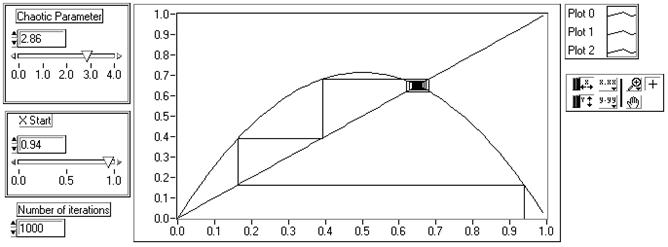
\includegraphics[width=0.65\linewidth]{images/Nldimage070.jpg}}
    \caption{Cob web analyzer shows the effect of repeatedly applying the quadratic map to the initial value $x$ = 0.94. It settles into a fixed point at about $x$ = 0.65}
    \label{fig:CobWebAnalyzer}
\end{figure}

The graph displays three plots. The downward parabola is the quadratic map $f(x) = rx(1-x)$. The straight line is $g(x) = x$, and the stair-step or ``cobweb'' is the effect of successively applying the quadratic map to the initial point, $x$ = 0.94 . The recipe for producing the cobweb is as follows: Begin with the initial point $x_0$, follow a vertical line up to $f(x_0)$, follow a horizontal line over to the line $y = x$, you are now at the x-coordinate $f(x_0)$, proceed vertically to the graph of the quadratic map. You are now at the y-coordinate $f(f(x_0))$ Each time you move vertically to $f$, you have performed a further iteration of the map. Continuing in this way you can explore the long-term behavior of the map as you vary the initial condition and the chaotic parameter.

Making this VI yourself will teach you about arrays, or lists of numbers, in LabView. If you haven't programmed in a computer language before, you should know that each number in an array is indexed starting from 0 to $N-1$. Here's the part of the cobweb VI that produces the graphs of $f$ and $g$ (Figure~\ref{fig:SectionOfCobWebVI}).

\begin{figure}[h]
    \centering
    \href{http://experimentationlab.berkeley.edu/sites/default/files/images/Nldimage082.gif}{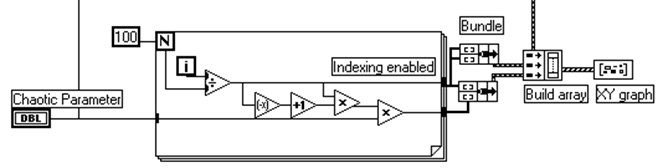
\includegraphics[width=0.7\linewidth]{images/Nldimage082.png}}
    \caption{Section of the cob web VI}
    \label{fig:SectionOfCobWebVI}
\end{figure}

The big square is a for-loop that gets executed 100 times (the constant 100 wired to N). Each time through the loop the variable \emph{i} increases by 1 (\emph{i} starts at zero and goes through \emph{(N-1)}). The quotient is calculated and assembled into an array, which we shall call $x_i$, at the right border of the loop. The function $f(x_i)$ is computed and also accumulated. The array is accumulated by means of the ``indexing'' feature at the border of the loop. Whenever you connect a wire from the inside to the outside of a loop a border node is formed to control how the data flows. Pop-up on the node to enable ``indexing'' and the result of each iteration will be assembled into an array. Leave indexing off and only the single number that was calculated last will be passed on.

Outside the loop, the arrays are ``bundled'' into a form that the XY-graph module will accept: an array of x-values bundled with an array of corresponding y-values. A ``bundle'' is a LabView data-structure that is a convenient way of collecting several things into one. It basically creates a list of ordered pairs, $\{x_i,y_i\}$ which the program then builds into an array with three such lists. The graph reads these three lists of ordered pairs and plays connect the dots, making three graphs. One graph is made by taking the $x_i$ array and bundling it with itself, producing the graph of y =x. The downward parabola, $y = rx(1-x)$, is made by bundling $x_i$ with $f(x_i)$.

That was the easy part, the graph of the cobweb part is a little harder and requires some discussion beforehand. We've already written a VI, named quad.vi, that calculates successive iterates of the quad map. The VI is located in C:\textbackslash NLD-chaos\textbackslash LABVIEW\textbackslash CHAOS. So let's assume we have a series of map-iterates
\[
    m_i = \{m_0,m_1,m_2, \cdots ,m_n\} = \{x_i,f(x_i),f(f(x_i)),\cdots f^n(x_i)\}
\]
We arrange these values in a way that will let LabView draw the cobweb by connecting the points:
\[
    \{x_i,y_i\} = \{(m_0,0),(m_0,m_1),(m_1,m_1),(m_1,m_2),(m_2,m_2),(m_2,m_3),\cdots (m_{n-1},m_{n-1}),(m_{n-1},m_n)\}
\]
The $x$-values form a series $\{m_0,m_0,m_1,m_1km_2,m_2,\cdots,m_{n-1},m_{n-1}\}$ which we may form by ``interleaving'' the $x_i$ array with itself and removing the last two elements. Fortunately, LabView has a function that interleaves arrays and a function that takes an array's subset.

The y-values of the cobweb form a series $\{0,m_1,m_1,m_2,m_2,\ldots ,m_{n-1},m_n\}$ which can also be made by interleaving the $x_i$ array and taking subsets (and replacing one element with a zero). Once you have the two arrays of $x$'s and $y$'s, you must bundle them together and then build an array out of this bundle and the other bundled plots of $f$ and $g$ (see the right side of Figure~\ref{fig:SectionOfCobWebVI}).

Try making the cobweb analyzer yourself. First, understand and make the section in Figure~\ref{fig:SectionOfCobWebVI}. Make the ``Build array'' icon have only two inputs, and then run the program. It should give you a graph of y =x and y =rx(1-x).

Next, expand the ``Build array'' icon to three inputs and start the cobweb part. Be sure to look at quad.vi to see how it works. You can add a VI into your diagram by going to the \emph{functions} palette and clicking ``Selecting a VI...''. You can then treat it as any other module with inputs and outputs. Consequently, all of the inputs in quad.vi will need to show up on your \emph{front-panel} except for the \emph{pre-iterate} input which you should just wire with a zero in your diagram. There are lots of different ways to program the cobweb, but you'll probably find the array functions ``Build Array,'' ``Interleave 1-D Arrays,'' ``Replace Array Elements,'' ``Array Size,'' and ``Array Subset'' helpful. Read what these modules do, and then make a block diagram on paper illustrating how you would use these functions to make the necessary x and y arrays for the cobweb. Then wire it up in LabView, bundle them together as before, and input it into the ``Build Array'' next to the other two bundles. Be sure to pay attention to whether your inputs/outputs are single elements or arrays of many elements. Some of the module inputs need to be told whether to accept elements or arrays.

Again, try to do this on your own. If you get really stuck, you can look in appendix A of this write-up for hints. Once you have the working VI, you can use it for a variety of things. Observe how the derivative of $f(x_i)$ affects the stability of fixed points (Ref.~\cite{Strogatz} \S10.1). Look for limit cycles, period windows, etc. Change the function $f(x_i)$ to $f(f(x_i))$ or some other 1-d map and observe the same qualitative behavior. To do this, you will have to modify both your program and quad.vi. Save quad.vi as quad2.vi in your directory rather than messing with the original. Try any non-invertible function that takes the unit interval to itself. There are numerous ones in the references: the tent map, the shift map, the sine map, etc. Try to come up with one of your own. Pretty much any function with a range of the unit interval that starts at (0,0) and goes to (1,0) will work. The maps must be non-invertible because there must be some dissipation in the equations [Ott \cite{Ott} p8]. Try at least one other map and analyze it.

\textbf{This is a Checkpoint: Call over a GSI and Professor and show them your program. Explain what you have done.}

\subsection{Numerical calculation of Liapunov Exponents}

Sensitive dependence on initial conditions is one of the defining features of chaotic behavior. Consider two close initial-conditions, $\xi$ and $\xi + \delta$ evolving in time. If their distance of separation increases exponentially, i.e. $|f(t,\xi) - f(t,\xi + \delta)| = \delta e^{\lambda t} $, we say the function $f$ exhibits sensitive dependence on initial conditions. The coefficient is necessarily positive and it is called the Liapunov exponent (see Ref.~\cite{Strogatz}, section 9.3 especially the qualifications after fig 9.3.5). As such, if you can calculate or measure , you have a test to determine whether or not a particular system is chaotic. If is not positive, the system is not chaotic.

As previously mentioned, the Liapunov exponents of multi-dimensional systems are the average eigenvalues of the Jacobian matrix of the system (see also Theiler \cite{Theiler} eq's 4-7). So rather than solving an eigenvalue problem on a multi-dimensional system, it's easier to start with a one-dimensional map. The Liapunov exponent for a 1-d map is given by (Ref.~\cite{Strogatz}, p367). Following example 10.5.3 in Ref.~\cite{Strogatz}, write a VI to calculate the Liapunov exponent of the quadratic map as a function of its chaotic parameter . You will probably find it useful to know that the inputs to LabView's arithmetic operators are \emph{polymorphic}. For example you can wire an array and a constant to the ``add'' function and the result is a new array whose elements are the old array with the constant added to each of them. Most of the math functions work this way for instance the log function can take an array of numbers and produce an array of logarithms of the numbers (see Figure 17). You will make use of quad.vi again.

\begin{figure}[h]
    \centering
    \href{http://experimentationlab.berkeley.edu/sites/default/files/images/Nldimage106.gif}{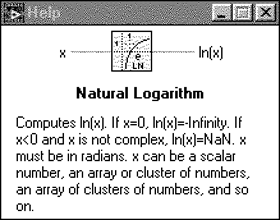
\includegraphics[width=0.5\linewidth]{images/Nldimage106.png}}
    \caption{LabView functions can take arrays as inputs, producing arrays of results.}
    \label{fig:Nldimage106}
\end{figure}

\begin{figure}[h]
    \centering
    \href{http://experimentationlab.berkeley.edu/sites/default/files/images/Nldimage107.gif}{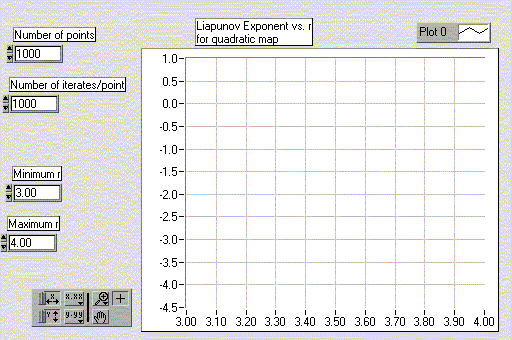
\includegraphics[width=0.5\linewidth]{images/Nldimage107.png}}
    \caption{Liapunov exponent VI.}
    \label{fig:Nldimage107}
\end{figure}

\newpage

The front panel of your finished VI should look something like Figure 18. After you look at the algorithm in Ref.~\cite{Strogatz}, make another block diagram of what you'll want to do and then try it in LabView. You'll probably find a FOR loop helpful. If you find yourself spending more than an hour or so on it, you should look at the solution in the appendix. When you have your working VI, explore the area around $r$ = 3.57 especially. What happens when $\lambda \rightarrow 0$ Use your observations to approximate Feigenbaum's ratio $\delta$. Ref.~\cite{Strogatz} suggests 10,000 iterations, but this is a bit excessive, not to mention time consuming. Make sure to have lots of different values for $r$, the chaotic parameter. Experiment to see what gives you good graphs.

\textbf{This is a Checkpoint: Call over a GSI and show them your program. Explain what you have done and which value of the chaotic parameter seems to work best.}

\subsection{NLSIM.VI: the simulation VI}

Before proceeding to real-time NLD systems, you will take some time to run the simulation VI, NLSIM.VI. Open NLSIM.VI. This VI (Figure~\ref{fig:SimulationVI}) allows you to display the time-series, return-map and power spectrum of a variety of signals. As in all the VI's, press control-H and move the mouse pointer over the elements of the screen to get specific information on how to use the program.

\begin{figure}[h]
    \centering
    \href{http://experimentationlab.berkeley.edu/sites/default/files/images/Nldimage109.gif}{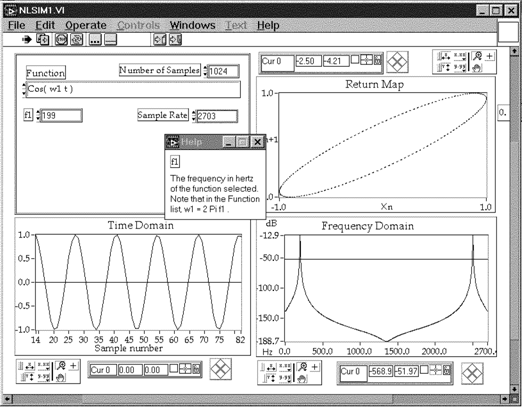
\includegraphics[width=0.7\linewidth]{images/Nldimage109.png}}
    \caption{The simulation VI.}
    \label{fig:SimulationVI}
\end{figure}

Start the VI, select the cosine function, and focus your attention to the return map. Many dynamical systems are described by a cosine function, for example the simple harmonic oscillator of a mass on a spring: $x(t) = A \cos(\sqrt{\frac{\kappa}{m}}t)$. What are the axes of the phase space of this system? What is the shape of the paths in phase space for this system? Is it similar to what you see in the return map? What effect does changing the sample rate have on the shape of the trajectory? When you increase the sample rate, why does the return map narrow around the line $y = x$? What happens if the sample rate is a multiple of the frequency of the cosine? Now try the function $\cos {(\omega_1t)} + \cos(\omega_2t) + a \cos(\omega_1t) \cos(\omega_2t)$. The return map for this function is more complicated: When $a$ is zero, it's a two-dimensional uncoupled harmonic oscillator and its trajectories are confined to a torus in phase space (c.f. Ref.~\cite{Strogatz}, \S8.6). What conditions are necessary for the return-map to show a projection of a torus and not a cycloid? Be sure to explain what you're seeing in the Time Domain and Frequency Domain. Is it chaotic?

Now select the Quadratic Map function and set the parameter $r$ = 2.8. The return map should show a single point. Increase $r$ to about 3, the map will bifurcate, and you should see two points on the return map. Continuing to increase $r$ will produce successive bifurcations and finally chaos at $r$ = 3.5. One dimensional maps like this one are good analogs to \emph{Poincaré sections} and when you sample the real NLD systems synchronous to their driving forces, you will see the same behavior. So it pays to spend some time here to really figure out what's going on. Be sure to compare this map with your cobweb VI at the same value of $r$. Also look at the quadratic map's bifurcation program.

\textbf{This is a Checkmark: Take a look at the Henon Map. Play with the non-linear parameter between 0 and about 1.4. What is that funky thing in the Return Map? Look at the Henon map's bifurcation program as well. Discuss what you are thinking with a GSI or Professor.}

\subsection{Continuous-time systems- PN Junction}

Now we're ready to proceed to real-time continuous systems. At present there are two driven NLD systems at the experiment station: The bouncing ball circuit and the PN-junction. For both these driven systems, the basic set-up is the same: The computer controls the driving amplitude and measures the system's response. Both circuits, as well as most of the supporting electronics are located behind the large panel marked ``Nonlinear Dynamics Laboratory.'' (see Figure~\ref{fig:NonlinearDynamicsLaboratoryPanel}) Note: the Sine Input switch should be off for the PN-junction part.

\begin{figure}[h]
    \centering
    \href{http://experimentationlab.berkeley.edu/sites/default/files/images/Nldimage115.gif}{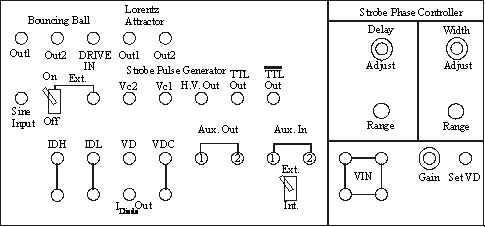
\includegraphics[width=0.7\linewidth]{images/Nldimage115.png}}
    \caption{The Physics 111-Lab Nonlinear Dynamics Laboratory Panel.}
    \label{fig:NonlinearDynamicsLaboratoryPanel}
\end{figure}

The drive oscillator is an Stanford Research System Model DS345. It is fed into the external reference pin $V_\text{ref}$ of the DAC on the computer. Recall from your basic electronics experience that when you set a DAC to a specific level, e.g. $j$ out of a maximum of $N$, the DAC outputs a voltage equal to $V_\text{DAC} = V_\text{ref} \frac{j}{N}$. Thus if $V_\text{ref}$ is a sine-wave varying in time, the DAC outputs a sine wave of attenuated amplitude. The computer modified sine-wave is then fed to the NLD system under study. The NLD system's response is sent to the ADC input of the computer where it can be sampled either synchronously or asynchronously with respect to the driving frequency. When sampling is performed asynchronously, an internal timebase (not shown) is used. Synchronous sampling is achieved by a ``strober,'' which sends TTL pulses to the EXTERNAL TRIGGER pin of the ADC whenever the drive signal achieves a certain phase (adjustable as ``Pulse delay'' on the NLD box) in its cycle. The sine-wave is also connected (via the square-wave converter on the NLD box) to the computer's timer pin (labeled GATE0) for computer measurement of the drive frequency.

\begin{figure}[h]
    \centering
    \href{http://experimentationlab.berkeley.edu/sites/default/files/images/Nldimage120.png}{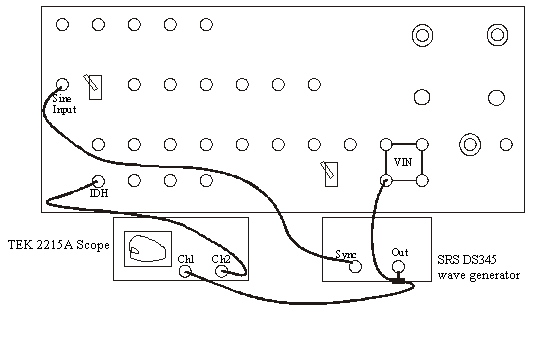
\includegraphics[width=0.7\linewidth]{images/Nldimage120.png}}
    \caption{Connecting the scope to see the phase portrait of the PN-junction.}
    \label{fig:ConnectingTheScope}
\end{figure}

The PN junction circuit requires power, so turn on the system with the switch on the power supply located at the top of the rack. Note: You should hook up the TTL bar output to the Z-axis input on the back of the scope. You will also need to have the Sine Input Switch Off.

Let's begin with the PN Junction: Make the following connections referring, in addition to Figure~\ref{fig:ConnectingTheScope}:

\newpage

\begin{itemize}
    \item $\overline{\text{TTL}}$ to the back of the Tektronix Dual Trace 2215A \href{http://physics111.lib.berkeley.edu/Physics111/Reprints/NLD/NLD_Equipment/01-2215scope.pdf}{scope}

    \item Set the SRS DS345 to $f$ = 3500 Hz and 10 volts, VPP output, Terminate with $50\Omega$.

    \item Set the STROBE PHASE CONTROLLER ``DELAY RANGE'' to 30 $\mu$s and ``ADJ'' to 0.0 (fully CCW)2

    \item Set the STROBE PHASE CONTROLLER ``WIDTH RANGE'' to 3 $\mu$s and ``ADJ'' to 0.0 (fully CCW)

    \item Set PN JUNCTION DRIVER ``GAIN'' to 0.0 (fully CCW).

\end{itemize}

You should now see a horizontal line on the scope. Increase the PN JUNCTION DRIVER GAIN and the scope should display an ellipse. Having connected $ V_o(t) $ and $ V_s(t) $ (recall the notation of the introduction) to the $x$, $y$ axes of the oscilloscope(remember to put the time dial on x.y). The displayed graph is a plot of $I$ vs. $V_{os} \cos(\theta)$, a two-dimensional projection of the system's path in phase space.

At such a low driving amplitude, the diode is responding linearly: The diode current is periodic at the same frequency as the drive oscillator with a small phase offset. Observe the behavior as you increase the DRIVER GAIN- it should follow the discussion of the pn-junction earlier in this write-up and the video.

The scope highlights sections of the plot according to the STROBE PHASE CONTROLLER adjustments. Hook up the TTL bar output to the Z-axis input on the back of the scope. Make sure the scope intensity is not too bright and you should be able to see the dots corresponding to points of constant phase of the drive. Recall that the state-space for this system is $(I, V_d,\theta)$ so a set of points sampled at a constant $\theta$ constitute a \textbf{Poincaré section}, a a subset of state space that slices the attractor non-tangential to the trajectories. The Poincaré section will contain as many dots as there are loops. Changing the DELAY potentiometer moves the slice along the attractor. When you sample asynchronously, the computer will sample coincident with the dots.

Now let's include the computer. All of the connections to the computer are made through a single box, called the \emph{Computer Interface Box} (Figure~\ref{fig:ConnectionsOnComputerInterfaceBox}).

\begin{figure}[h]
    \centering
    \href{http://experimentationlab.berkeley.edu/sites/default/files/images/NLD_DAQBOX.png}{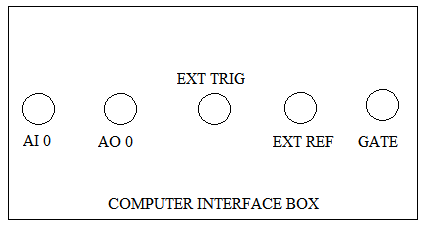
\includegraphics[width=0.5\linewidth]{images/NLD_DAQBOX.png}}
    \caption{The connections on the computer interface box.}
    \label{fig:ConnectionsOnComputerInterfaceBox}
\end{figure}

Disconnect the SRS DS345 from Vin and make the following connections, in addition to looking at Figure~\ref{fig:ConnectionsForComputerSamplingOfPNJunction}. $V_{os} \cos(\theta)$,

\newpage

\begin{itemize}
    \item SRS DS345 ``$ 50 \Omega $; Sine output ----------------------------to ``EXT REF''

    \item COMPUTER ``AO 0''-----------------------------------------to PN JUNCTION ``$V_{in}$''

    \item PN JUNCTION ``Differential $I_{diode}$ out''---------------to ``AI 0''

    \item STROBE PULSE GENERATOR ``TTL OUT''-------------to ``GATE''

    \item STROBE PULSE GENERATOR ``TTL OUT''-------------to ``EXT TRIG''

    \item Sine Input switch set to -----------------------------------Off

    \item set the switch below AUX in/out ---------------------to ``INT''
\end{itemize}

\begin{figure}[h]
    \centering
    \href{http://experimentationlab.berkeley.edu/sites/default/files/images/NLD_PN_DIAGRAM.png}{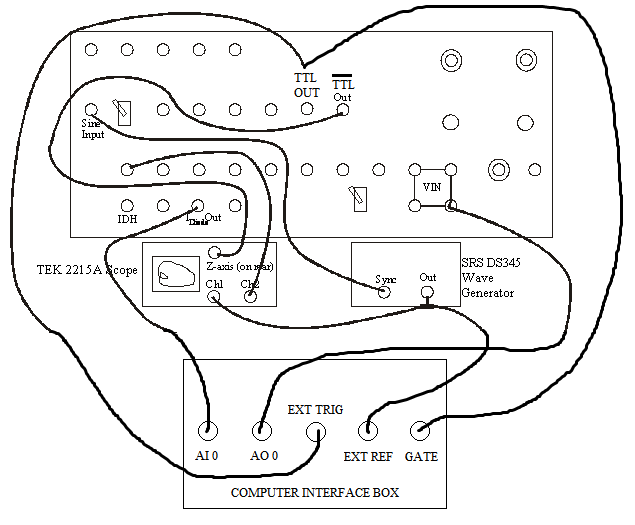
\includegraphics[width=0.7\linewidth]{images/NLD_PN_DIAGRAM.png}}
    \caption{Connections for computer sampling of the PN-junction.}
    \label{fig:ConnectionsForComputerSamplingOfPNJunction}
\end{figure}

Start LabView and load NLDGEN. You should see a display similar to Figure~\ref{fig:NLDGENVI}.

\begin{figure}[h]
    \centering
    \href{http://experimentationlab.berkeley.edu/sites/default/files/images/Nldimage128.gif}{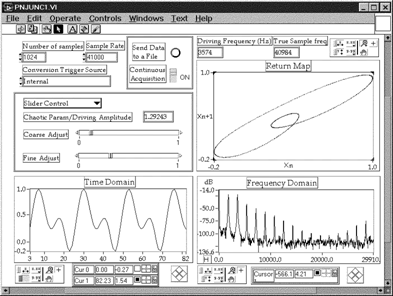
\includegraphics[width=0.5\linewidth]{images/Nldimage128.png}}
    \caption{NLDGEN.VI (similar to pnjunc1.vi)- For sampling real-time driven NLD systems.}
    \label{fig:NLDGENVI}
\end{figure}

This VI controls the drive amplitude, collects a sample of data points, and presents three different views of the response: a time-series, Fourier power spectrum, and return-map. We suggest you use ~30kHz for the sampling rate. The more points you take in your sample, the better your DFT resolution will be, but the longer the computer will take to calculate and display. So to start, select 256 points. \textbf{You should make sure that the product of ``Number of points per value of V'' and ``\#'' of points" does not exceed $2^{31} - 1$.}  Vary the drive amplitude and estimate Feigenbaum's ratio based on the system's bifurcation points. Compare the return map to the picture you see on the scope. There are two other features of this VI: You can save the data to a file, and send the data to a subroutine that calculates information dimension. We'll discuss these options later.

Before moving on, open up nldbifur.vi, which will allow you to view the bifurcation diagram for the PN-junction. Leave the computer and hardware in the same configuration as for nldgen.vi, except turn the knob for PN-JUNCTION DRIVER GAIN all the way up (CW). You should also look at the real-time output on the scope, so also hook the output on the SRS DS345 to the X-channel on the scope, and the IDH output on the PN-JUNCTION DRIVER into the Y-channel, just as before. Run nldbifur.vi and look at several different ranges of V.

\section{Bouncing Ball}

Let's now turn our attention to the bouncing ball circuit (BB).

\begin{figure}[h]
    \centering
    \href{http://experimentationlab.berkeley.edu/sites/default/files/images/Nldimage130.png}{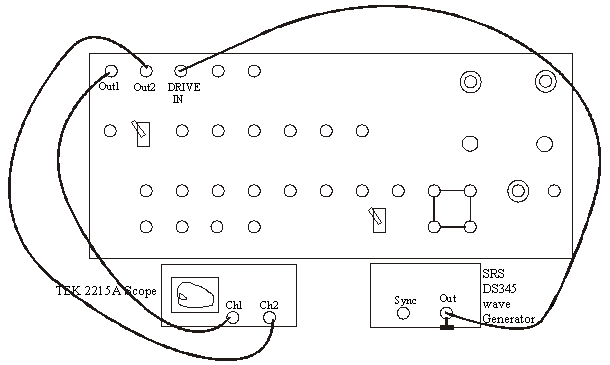
\includegraphics[width=0.7\linewidth]{images/Nldimage130.png}}
    \caption{Connections for Bouncing Ball Circuit.}
    \label{fig:ConnectionsForBouncingBallCircuit}
\end{figure}

\begin{itemize}
    \item Connect the SRS DS345 Sine out to the DRIVE input on the panel.

    \item Connect BB OUT1 to the Tek 2215 scope CH 1.

    \item Connect BB OUT2 to the Tek 2215 scope CH 2.
\end{itemize}

\newpage

Set the DS345 to  $\sim$50Hz and  $\sim$10V peak-to-peak (just turn the knob to about half-way in its range). Look at each channel in time. They should both be sinusoids. Put the scope in X-Y mode and you will see the system's phase portrait. The circuit is fully described in the reprints so we will only summarize it here: The circuit simulates the dynamics of a ball bouncing on a vertically sinusoidally driven table. One output is ball velocity, one is ball position (height from a fixed reference). When the table frequency and amplitude are small, the ball basically stays on the table and the phase portrait is that of an harmonic oscillator. Increase the drive frequency and you should see the phase-portrait begin to change. The phase-portrait becomes jittery and then it should jump to behavior that is periodic at twice the drive frequency. Take some time to understand the simple behaviors of the phase portrait: Which axis is velocity? Which is position? Why is the initial plot an ellipse? What's happening just as you increase the drive frequency but before the plot becomes jittery? Try varying the drive voltage.

Now we're ready to hook up the computer. Make/check the following connections, referring to Figure~\ref{fig:ConnectionsForBouncingBallCircuitToComputer}:

\begin{figure}[h]
    \centering
    \href{http://experimentationlab.berkeley.edu/sites/default/files/images/NLD_BALL_DIAGRAM.png}{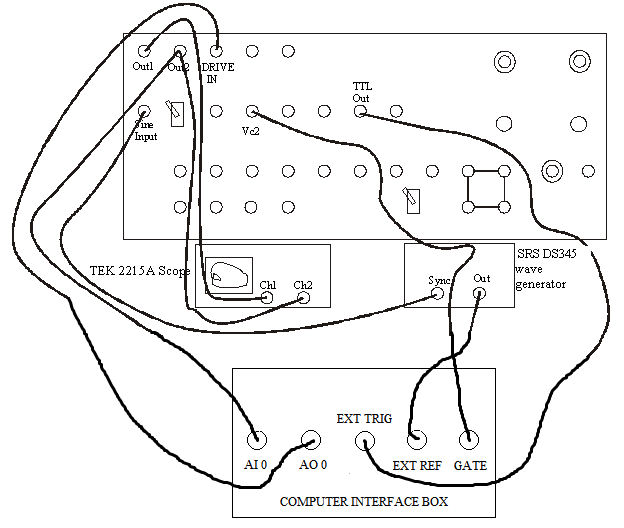
\includegraphics[width=0.5\linewidth]{images/NLD_BALL_DIAGRAM.png}}
    \caption{Connections for Bouncing Ball Circuit to the computer.}
    \label{fig:ConnectionsForBouncingBallCircuitToComputer}
\end{figure}

\begin{itemize}
    \item Disconnect the PN-JUNCTION setup

\end{itemize}

Connect . . .

\begin{itemize}
    \item DS345 ``Sine output''---------------- to ``EXT REF''

    \item DS345 ``Sync out''------------------- to STROBE PULSE GENERATOR ``SINE INPUT''

    \item ``AO 0''--------------------------------- to Bouncing ball ``DRIVE''

    \item Bouncing ball OUT 1--------------- to scope CH1

    \item Bouncing ball OUT 2--------------- to scope CH2 and ``AI 0''

    \item STROBE PULSE GENERATOR ``VC2''-------- to ``GATE''

    \item STROBE PULSE GENERATOR ``TTL OUT''- to ``EXT TRIG''

    \item Set the Sine Input Swtich to---------------------------Off

    \item Set the DS345 to $f$ = 90Hz and full amplitude output.

    \item Run the NLDGEN VI and start by sampling 256 points at 500 Hz
\end{itemize}

\textbf{This is a Checkpoint: What is fundamentally different about the chaotic behavior of the bouncing ball circuit when compared to the PN-Junction? (Hint: What would the bifurcation diagram for this circuit look like? Does it even have one?) Discuss what you notice with a Professor or GSI.}

\subsection{Information dimension}

\begin{figure}[h]
    \centering
    \href{http://experimentationlab.berkeley.edu/sites/default/files/images/180px-Nldimage133.gif}{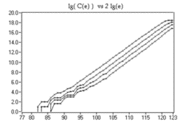
\includegraphics[width=0.5\linewidth]{images/180px-Nldimage133.png}}
    \caption{Data from the Quadratic map, analyzed by the information-dimension VI.}
    \label{fig:DataFromQuadraticMap}
\end{figure}

Chaotic systems have fractal attractors and a commonly measured quantity is the attractor's information (or correlation) dimension (Ref.~\cite{Strogatz}, \S11.5, Ref.~\cite{Theiler}, pp1062-1063, pp1066-1070). The correlation dimension measures how the state-space ``mass'' of the attractor scales with length. CALCCORR.VI computes $C(N,\epsilon)$, the number of points within a distance $\epsilon$ of each other, for increasing embedding dimensions and then displays $\log_2 C(N,\epsilon)$ vs. $2 \log_2 \epsilon$ (Figure~\ref{fig:DataFromQuadraticMap}). The slope of the linear region of the plot is then 1/2 times the information dimension. See the article by Theiler \cite{Theiler} for full details and Ref.~\cite{Buskirk} for a simple application of these concepts.

\begin{itemize}
    \item As an introductory exercise, do the following: Run NLSIM.VI and CALCCORR.VI. Select ``Random number generator.'' Choose 2048 points and press the ``Send data to the info-dimension VI'' button. Press ``Calculate'' in CALCORR. When the calculation is done, use the graph cursors to estimate the slope of each line. How does each slope compare to the line's embedding-dimension?
\end{itemize}

The data calculated by CALCCORR.VI can be saved to a data file for more accurate linear fitting. Simply press the ``send data to a file'' button, name the file, and open it from within Excel (or copy it to a disk and take it to your favorite software). You should measure the information dimension of the PN-junction and the Bouncing Ball circuit for varying driving amplitudes and frequencies. Are the values what you expect?

\section{What your report should contain}

Your report should be an introduction to NLD and Chaos and a presentation of experimental results. Most of this material about chaos is unfamiliar to the majority of undergraduates. Thus your goal should be to illustrate the concepts set forth in the reading by relating them to what you did in lab.

The results you should present are \emph{at least} the following: Experimental confirmation of the bifurcation route to chaos. The value of Feigenbaum's scaling constant $\alpha$ and $\delta$ measured from a variety of sources. What does Feigenbaum's ratio mean? The information (Lyapunov) dimension of the attractors of the PN-junction and the Bouncing Ball circuit as compared to that of conservative (Hamiltonian) systems. How do the Fourier Transform, the frequency spectrum, and the power spectrum differ?

Be sure to answer the questions posed in the write-up and include your answers to the pre-lab.

\begin{itemize}
    \item Last day of the experiment please fill out the \href{\ExperimentEvaluation}{\textbf{Experiment Evaluation}}

\end{itemize}

\section{The Custom VI's for this experiment}

Henonbifr.VI Illustrates bifurcation in one of the variables of the Henon map.

Henon.VI Iterates the Henon map

NLSim.VI Displays time-series, return maps, and Fourier spectrum of many simulated signals and an arbitrarily acquired signal

PNJunc1.VI Acquires and analyzes time-series data acquired from the PN junction

NLDBifur.VI.

Quad.VI Iterates the quadratic map.

QuadBifr.VI Calculates the bifurcation diagram for the quadratic map.

\begin{figure}[h]
    \centering
    \href{http://experimentationlab.berkeley.edu/sites/default/files/images/Nldimage138.gif}{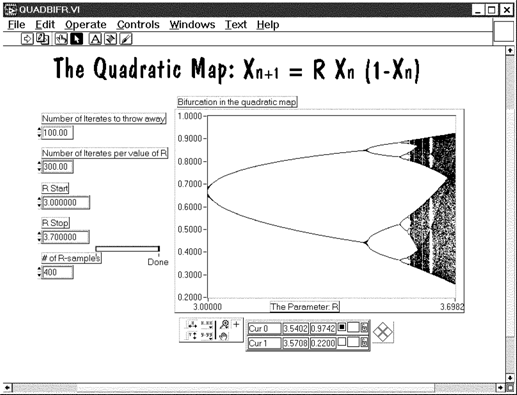
\includegraphics[width=0.6\linewidth]{images/Nldimage138.png}}
    \caption{\textbf{Quad Bifur} This VI permits you to explore the Bifurcation diagram of the quadratic map. You can change the parameters to reveal the fine detail at the onset of chaos.}
\end{figure}

\begin{figure}[h]
    \centering
    \href{http://experimentationlab.berkeley.edu/sites/default/files/images/Nldimage139.gif}{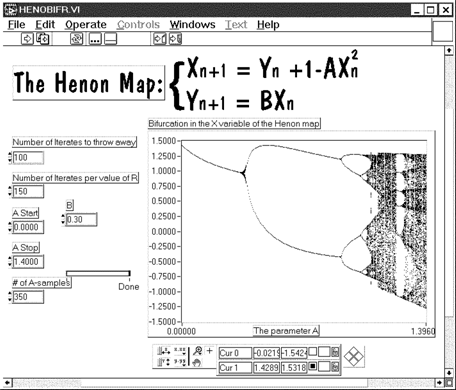
\includegraphics[width=0.5\linewidth]{images/Nldimage139.png}}
    \caption{\textbf{Henon Bifur}}
\end{figure}

\begin{figure}[h]
    \centering
    \href{http://experimentationlab.berkeley.edu/sites/default/files/images/Nldimage140.gif}{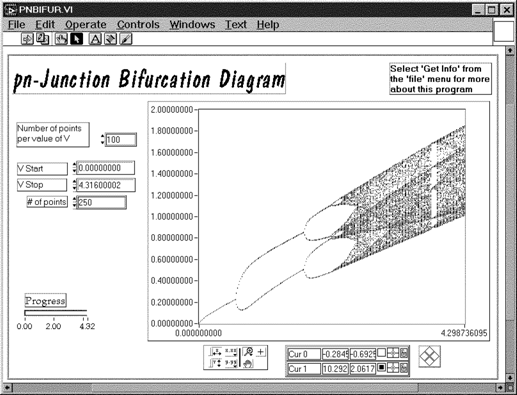
\includegraphics[width=0.5\linewidth]{images/Nldimage140.png}}
    \caption{\textbf{NLDBifur}}
\end{figure}

\appendix

\begin{figure}[h]
    \centering
    \href{http://experimentationlab.berkeley.edu/sites/default/files/images/Nldimage141.gif}{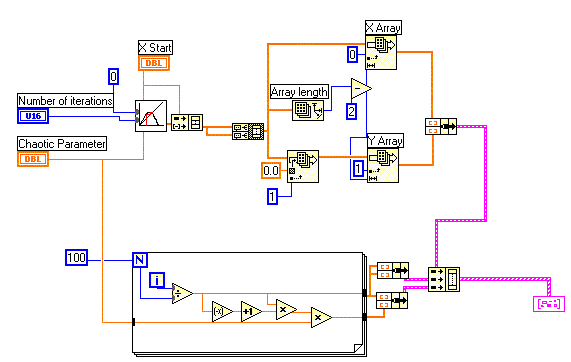
\includegraphics[width=\linewidth]{images/Nldimage141.png}}
    \caption{Cobweb analyzer for the quadratic map. \textbf{Cobweb2.vi}}
\end{figure}

\textbf{Note: The elements in the current LabView program VI do not look quite like the elements in these diagrams.}

\begin{figure}[h]
    \centering
    \href{http://experimentationlab.berkeley.edu/sites/default/files/images/Nldimage142.jpg}{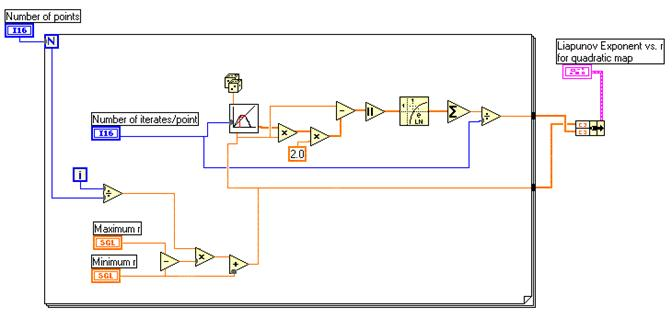
\includegraphics[width=\linewidth]{images/Nldimage142.jpg}}
    \caption{Liapunov exponent VI. \textbf{liapunov2.vi}}
\end{figure}

\end{document}
